\chapter{Operations on stable functions}
\label{chap:operations}

Having identified several classes of stable Generalized Density Functions (GDFs)
in Chapter~\ref{chap:stable_functions}, we now turn to a natural subsequent
question: \emph{how does stability behave under common operations?}
If we combine stable GDFs, for instance, by pointwise addition or by taking
their minimum, is the resulting GDF also stable? If so, can we bound its
stability constant in terms of the constants of the original functions? This
chapter explores these questions, identifying conditions under which stability
is preserved and providing counterexamples where it is not. Understanding these
properties is crucial for constructing more complex stable GDFs from simpler
ones and for gaining deeper insight into the structure of the space of stable
functions.

\section{Affine transformations}

We begin with the simplest operations: adding a constant to a stable GDF and
multiplying it by a constant.

\begin{theorem}[Stability under constant addition]
    \label{thm:constant_addition}
    Let $f(P, x)$ be a $c$-stable GDF with $q$-tame induced persistence modules.
    Then, for any constant $z \in \mathbb{R}$, the GDF
    $g(P, x) = f(P, x) + z$ is also $c$-stable with $q$-tame induced
    persistence modules.
\end{theorem}
\begin{proof}
    \begin{figure}
        \centering
        \pgfmathsetmacro{\off}{6.5}
        \pgfmathsetmacro{\z}{1.3}
        \hspace*{-1cm}
        \begin{tikzpicture}
            \small
            % Axes
            \draw[->] (0,0) -- (5,0) node[right] {Birth};
            \draw[->] (0,0) -- (0,5.5) node[above] {Death};
            \draw[->] ({\off},0) -- ({6+\off},0) node[right] {Birth};
            \draw[->] ({\off},0) -- ({\off},5.5) node[above] {Death};
            
            % Grid
            % \draw[gray!30] (0,0) grid (6,6);
            
            % Diagonal
            \draw[dashed] (0,0) -- (5,5);
            \draw[dashed] ({\off},0) -- ({5+\off},5);
            
            % Point coords
            \coordinate (p1) at (1.3,3);
            \coordinate (p1z) at ($(p1) + (\z,\z)$);
            \coordinate (p2) at (0.8,1.3);
            \coordinate (p2z) at ($(p2) + (\z,\z)$);
            \coordinate (p3) at (3,5);
            \coordinate (p3z) at ($(p3) + (\z,0)$);
            
            \coordinate (q1) at ({\off + 1.1},2.6);
            \coordinate (q1z) at ($(q1) + (\z,\z)$);
            \coordinate (q2) at ({\off + 1},1);
            \coordinate (q2z) at ($(q2) + (\z,\z)$);
            \coordinate (q3) at ({\off + 2.5},5);
            \coordinate (q3z) at ($(q3) + (\z,0)$);
            
            % Lines to axes
            % \draw[dashed,gray] (p1) -- (p1 |- 0,0) node[below,blue,rotate=45,anchor=east] {$b_1$};
            % \draw[dashed,gray] (p1) -- (0,0 |- p1) node[left,blue] {$d_1$};
            % \draw[dashed,gray] (p1z) -- (p1z |- 0,0) node[below,red,rotate=45,anchor=east] {$b_1+z$};
            % \draw[dashed,gray] (p1z) -- (0,0 |- p1z) node[left,red] {$d_1+z$};
            % \draw[dashed,gray] (p2) -- (p2 |- 0,0) node[below,blue,rotate=45,anchor=east] {$b_2$};
            % \draw[dashed,gray] (p2) -- (0,0 |- p2) node[left,blue] {$d_2$};
            % \draw[dashed,gray] (p2z) -- (p2z |- 0,0) node[below,red,rotate=45,anchor=east] {$b_2+z$};
            % \draw[dashed,gray] (p2z) -- (0,0 |- p2z) node[left,red] {$d_2+z$};
            % \draw[dashed,gray] (p3) -- (p3 |- 0,0) node[below,blue,rotate=45,anchor=east] {$b_3$};
            % \draw[dashed,gray] (p3z) -- (p3z |- 0,0) node[below,red,rotate=45,anchor=east] {$b_3+z$};
            % \draw[dashed,gray] (5,5) -- (0,5) node[left,black] {$\infty$};

            % Points
            \fill[blue] (p1) circle (2pt) node[above left,blue] {$p_1$};
            \fill[blue] (p2) circle (2pt) node[above left,blue] {$p_2$};
            \fill[blue] (p3) circle (2pt) node[above left,blue] {$p_3$};
            \fill[red] (p1z) circle (2pt) node[above left,red] {$p_1+z$};
            \fill[red] (p2z) circle (2pt) node[above right,red] {$p_2+z$};
            \fill[red] (p3z) circle (2pt) node[above left,red] {$p_3+z$};

            \fill[blue] (q1) circle (2pt) node[above right,blue] {$q_1$};
            \fill[blue] (q2) circle (2pt) node[below right,blue] {$q_2$};
            \fill[blue] (q3) circle (2pt) node[above left,blue] {$q_3$};
            \fill[red] (q1z) circle (2pt) node[above right,red] {$q_1+z$};
            \fill[red] (q2z) circle (2pt) node[below right,red] {$q_2+z$};
            \fill[red] (q3z) circle (2pt) node[above right,red] {$q_3+z$};
            
            \path[blue, bend left, shorten <= 0.15cm, shorten >= 0.15cm] (p1) edge (q1);
            \path[blue, bend right=20, shorten <= 0.15cm, shorten >= 0.15cm] (p2) edge (q2);
            \path[blue, bend right, shorten <= 0.15cm, shorten >= 0.15cm] (p3) edge (q3);
            \path[red, bend right=10, shorten <= 0.15cm, shorten >= 0.15cm] (p1z) edge (q1z);
            \path[red, bend right=20, shorten <= 0.15cm, shorten >= 0.15cm] (p2z) edge (q2z);
            \path[red, bend left, shorten <= 0.15cm, shorten >= 0.15cm] (p3z) edge (q3z);
        \end{tikzpicture}
        \caption{
            The persistence diagrams of $f_P$ (left, blue), $f_Q$ (right, blue),
            and $g_P$ (left, red), $g_Q$ (right, red) where $g_P = f_P + z$ and
            $g_Q = f_Q + z$. A matching between the diagrams of $f_P$ and
            $f_Q$ is shown in blue, and a matching between the diagrams of
            $g_P$ and $g_Q$ is shown in red.
        }
        \label{fig:constant_addition_pds}
    \end{figure}

    First we related the sublevel sets of $g_P$ and $f_P$.
    For any $a \in \R$:
    \begin{align}
        g^{-1}_P(-\infty, a] &= \{x \in \R^d \mid g_P(x) \leq a\} \\
        &= \{x \in \R^d \mid f_P(x) + z \leq a\} \\
        &= \{x \in \R^d \mid f_P(x) \leq a - z\} \\
        &= f^{-1}_P(-\infty, a - z].
    \end{align}
    This means the sublevel set filtration $\{g_P^{-1}(-\infty, a]\}_{a\in \R}$
    is identical to the filtration $\{f_P^{-1}(-\infty, b]\}_{b\in \R}$ but
    with the indices shifted by $z$, i.e., $b = a - z$.
    Consequently, if a topological feature is born at $b$ and dies at $d$ in
    the filtration of $f_P$, a corresponding feature in the filtration of $g_P$
    will be born at $b + z$ and die at $d + z$, and vice versa.
    Thus, the persistence diagrams of $f_P$ and $g_P$ are related by a constant
    shift along both axes:
    \begin{equation}
        \dgm_k(g_P) = \{(b + z, d + z) \mid (b, d) \in \dgm_k(f_P)\}.
    \end{equation}
    
    Next, we address $q$-tameness.
    Let $\mathbb{F} = (\{F_a\}, \{\mathfrak{f}_a^{a'}\})$ be a persistence
    module induced by $f_P$ and
    $\mathbb{G} = (\{G_a\}, \{\mathfrak{g}_a^{a'}\})$ be that induced by $g_P$.
    From the relationship between the sublevel sets, we have
    $G_a = F_{a - z}$ and $\mathfrak{g}_a^{a'} = \mathfrak{f}_{a - z}^{a' - z}$.
    Since $\mathbb{F}$ is $q$-tame by assumption, $\mathfrak{f}_a^{a'}$ is of
    finite rank for $b < b'$.
    This directly implies that $\mathfrak{g}_a^{a'}$ is also of finite rank for
    all $a < a'$, so $\mathbb{G}$ is also $q$-tame.
    
    Finally, we prove $c$-stability for $g$.
    Fix point clouds $P$ and $Q$.
    By stability of $f$, we have that
    \begin{equation}
        d_b(\dgm_k(f_P), \dgm_k(f_Q)) \leq c \cdot d_H(P, Q).
    \end{equation}
    Let $\pi_i$ be a sequence of matchings between $\dgm_k(f_P) \cup \Delta$ and
    $\dgm_k(f_Q) \cup \Delta$ that achieves this bound.
    For each $i$, we can construct a matching $\pi'_i$ between
    $\dgm_k(g_P) \cup \Delta$ and $\dgm_k(g_Q) \cup \Delta$ by shifting the
    points in $\pi_i$ by $z$:
    \begin{equation}
        \pi'_i(b + z, d + z) = (b' + z, d' + z) \text{ where } (b', d') = \pi_i(b, d).
    \end{equation}
    The cost of this matching is the same as that of $\pi_i$:
    \begin{equation}
        \norm{(b + z, d + z) - \pi'_i(b + z, d + z)}_\infty = \norm{(b, d) - (b', d')}_\infty,
    \end{equation}
    thus $\pi_i'$ is a matching between $\dgm_k(g_P)$ and $\dgm_k(g_Q)$ with the same
    cost as $\pi_i$. An example of this is shown in
    Figure~\ref{fig:constant_addition_pds}.
    Therefore, we have:
    \begin{equation}
        d_b(\dgm_k(g_P), \dgm_k(g_Q)) \leq c \cdot d_H(P, Q).
    \end{equation}
    Since this holds for arbitrary $P$ and $Q$, $g$ is $c$-stable.
\end{proof}

\begin{theorem}[Stability under positive constant multiplication]
    \label{thm:constant_nonneg_multiplication}
    Let $f(P, x)$ be a $c$-stable GDF with $q$-tame induced persistence modules.
    Then for any constant $\alpha \geq 0$, the function
    $g(P, x) = \alpha f(P, x)$ is also a $c\alpha$-stable GDF with
    $q$-tame induced persistence modules.
\end{theorem}
\begin{proof}
    We first consider the case when $\alpha = 0$.
    In this case, $g(P, x) = 0$ for all $x \in \R^d$, which is $0$-stable
    by Theorem~\ref{thm:independent_stable}. Its induced persistence modules
    are pointwise finite dimensional, hence $q$-tame.
    
    Now, let $\alpha > 0$.
    The argument mirrors that of Theorem~\ref{thm:constant_addition}.
    The sublevel sets of $g$ and of $f$ are related by:
    \begin{equation}
        g^{-1}_P(-\infty, a] = \{x \in \R^d \mid \alpha f_P(x) \leq a\} = f^{-1}_P(-\infty, a/\alpha].
    \end{equation}
    This implies that the persistence module $\mathbb{G}$ induced by $g_P$ is
    the same as the persistence module $\mathbb{F}$ induced by $f_P$ up to reindexing where $a$ is replaced with $a \cdot \alpha$, i.e.
    $F_a = G_{a \cdot \alpha}$ and the maps $\mathfrak{f}_a^{a'}$ and
    $\mathfrak{g}_{\alpha \cdot a}^{\alpha \cdot a'}$ are identical.
    The $q$-tameness of $\mathbb{F}$ implies the $q$-tameness of $\mathbb{G}$.

    A point $(b, d)\in \dgm_k(f_P)$ corresponds to $(\alpha b, \alpha d) \in
    \dgm_k(g_P)$ and vice versa. By the same argument as in the proof of
    Theorem~\ref{thm:constant_addition}, we can construct a matching
    $\pi'_i(b \cdot \alpha, d \cdot \alpha) = (b' \cdot \alpha, d' \cdot \alpha)$ where
    $(b', d') = \pi_i(b, d)$, which gives a bound on the bottleneck distance
    between the persistence diagrams of $g_P$ and $g_Q$:
    \begin{equation}
        d_b(\dgm_k(g_P), \dgm_k(g_Q)) \leq c \cdot \alpha \cdot d_H(P, Q).
    \end{equation}
\end{proof}

We can extend this theorem to negative constants using the following lemma:
\begin{lemma}[Stability under negation]
    \label{lem:negation_stability}
    Let $f(P, x)$ be a $c$-stable GDF with $q$-tame induced persistence modules.
    Then the function $g(P, x) = - f(P, x)$ is also a $c$-stable GDF
    with $q$-tame induced persistence modules.
\end{lemma}
\begin{proof}
    This is a direct consequence of the symmetry theorem by David Cohen-Steiner
    et al.~\cite{cohen2009extending}, which states that for a real-valued
    function $f$ on a $d$-manifold the persistence diagrams $\dgm_k(f)$ and
    $\dgm_{d - k}(-f)$ are reflections of each other across the minor diagonal.
    Given that $\R^d$ is a $d$-manifold and reflection preserves bottleneck
    distance, the lemma follows immediately.
\end{proof}

Combining Theorem~\ref{thm:constant_nonneg_multiplication} and
Lemma~\ref{lem:negation_stability}, we obtain the following corollary:
\begin{corollary}[Stability under constant multiplication]
    \label{cor:constant_multiplication}
    Let $f(P, x)$ be a $c$-stable GDF with $q$-tame induced persistence modules.
    Then for any constant $\alpha \in \mathbb{R}$, the function
    $g(P, x) = \alpha f(P, x)$ is also a $c|\alpha|$-stable GDF with
    $q$-tame induced persistence modules.
\end{corollary}

\section{Addition of stable functions}
\label{sec:addition_stable}

Having examined affine transformations, we now explore the effect of adding two
stable GDFs.
Let $f$ and $g$ be GDFs with stability constants $c_f$ and $c_g$.
What can be said about the stability constant of their sum
$h(P, x) = f(P, x) + g(P, x)$?
A simple case offers initial intuition:
if $g = f$, then $h = f + f = 2 \cdot f$.
By Theorem~\ref{thm:constant_addition}, $h$ is $(2 \cdot c_f)$-stable.
One would naturally expect that the stability constant of
$h = f + g$ is then bounded by $c_f + c_g$, but this is not always the case,
as the following example demonstrates.
\begin{example}[Sum of stable GDFs may not be stable]
    Consider GDFs on $\R$ ($d = 1$).
    Fix a constant $a > 0$, let
    \begin{equation}
        f(P, x) = x + a \cdot \min P \quad \text{and} \quad g(P, x) = - x + a \cdot \min P.
    \end{equation}
    As described in Example~\ref{ex:x_plus_g}, both GDFs are $0$-stable.

    The sum of $f$ and $g$ is:
    \begin{equation}
        h(P, x) = f(P, x) + g(P, x) = 2a \cdot \min P.
    \end{equation}
    The function $h_P$ is constant for a fixed $P$.
    Its 0-dimensional persistence diagram has exactly one point
    $(2a \cdot \min P, \infty)$, representing the single connected component
    $\R$ itself, born at $2a \cdot \min P$ and never dying.
    
    Let $P = \{1\}, Q = \{2\}$ with $d_H(P, Q) = 1$.
    The 0-dimensional persistence diagrams of $h$ are
    $\dgm_0(h_P) = \{(2a, \infty)\}$ and $\dgm_0(h_Q) = \{(4a, \infty)\}$.
    In the optimal matching $\pi$ between these diagrams, the point $(2a, \infty)$
    must be matched to $(4a, \infty)$, as matching either of them to the
    diagonal $\Delta$ would result in an infinite cost.
    The cost of $\pi$ is thus:
    \begin{equation}
        \norm{(2a, \infty) - (4a, \infty)}_\infty = 2a.
    \end{equation}
    Therefore, the bottleneck distance between the diagrams is $2a$,
    and for $h$ to be $c$-stable, we need:
    \begin{equation}
        2a \leq c \cdot d_H(P, Q) = c.
    \end{equation}
    This means that for any $c \in [0, \infty)$, we can choose $a = c$ such that
    the stability constant of $h$ is larger than $c$.
    Thus, the sum of two $0$-stable GDFs is not necessarily $c$-stable for
    any $c \in [0, \infty)$.
\end{example}

Despite this counterexample for general stable GDFs, stability under addition
holds for the more restrictive class of PC-Lipschitz GDFs.
\begin{theorem}[Sum of PC-Lipschitz GDFs]
    \label{thm:sum_pc_lipschitz}
    Let $f(P, x)$ and $g(P, x)$ be a $c_f$-PC-Lipschitz GDF and a
    $c_g$-PC-Lipschitz GDF. Then their sum $h(P, x) = f(P, x) + g(P, x)$ is
    a $(c_f + c_g)$-PC-Lipschitz GDF and is thus $(c_f + c_g)$-stable
    if the induced persistence modules of $h$ are $q$-tame.
\end{theorem}
\begin{proof}
    Let $P, Q \subseteq \R^d$ be finite point clouds.
    By subadditivity of the $\infty$-norm and the definition of
    PC-Lipschitz continuity, we have:
    \begin{align}
        \norm{h_P - h_Q}_\infty &= \norm{(f_P + g_P) - (f_Q + g_Q)}_\infty \\
        & \leq \norm{f_P - f_Q}_\infty + \norm{g_P - g_Q}_\infty \\
        & \leq c_f \cdot d_H(P, Q) + c_g \cdot d_H(P, Q) \\
        & = (c_f + c_g) \cdot d_H(P, Q),
    \end{align}
    which shows that $h$ is ($c_f + c_g$)PC-Lipschitz.
    By Lemma~\ref{lem:pc_lipschitz_stable}, $h$ is $(c_f + c_g)$-stable if its
    induced persistence modules are $q$-tame.
\end{proof}

\section{Minimum and maximum of stable functions}

Similar to addition, the pointwise minimum of two PC-Lipschitz GDFs is also
PC-Lipschitz, and thus stable.
\begin{theorem}[Minimum of PC-Lipschitz GDFs]
    \label{thm:min_pc_lipschitz}
    Let $f(P, x)$ and $g(P, x)$ be a $c_f$-PC-Lipschitz GDF and a
    $c_g$-PC-Lipschitz GDF.
    Then the function $h(P, x) = \min\{f(P, x), g(P, x)\}$
    is a $\max\{c_f, c_g\}$-PC-Lipschitz GDF and is thus $\max\{c_f, c_g\}$-stable
    if the induced persistence modules of $h$ are $q$-tame.
\end{theorem}
\begin{proof}
    This result follows directly from a standard property of Lipschitz
    functions: the pointwise minimum (or maximum) of two Lipschitz functions
    $F_1, F_2: X \to Y$ with Lipschitz constants $L_1, L_2$ is itself
    Lipschitz with constant $\max\{L_1, L_2\}$~(\cite{weaver2018lipschitz},
    Proposition~1.5.5).
\end{proof}

However, this property does not hold for general stable GDFs, as shown in the
following counterexample.
\begin{example}[Minimum of $0$-stable GDFs can be unstable]
    \begin{figure}
        \centering
        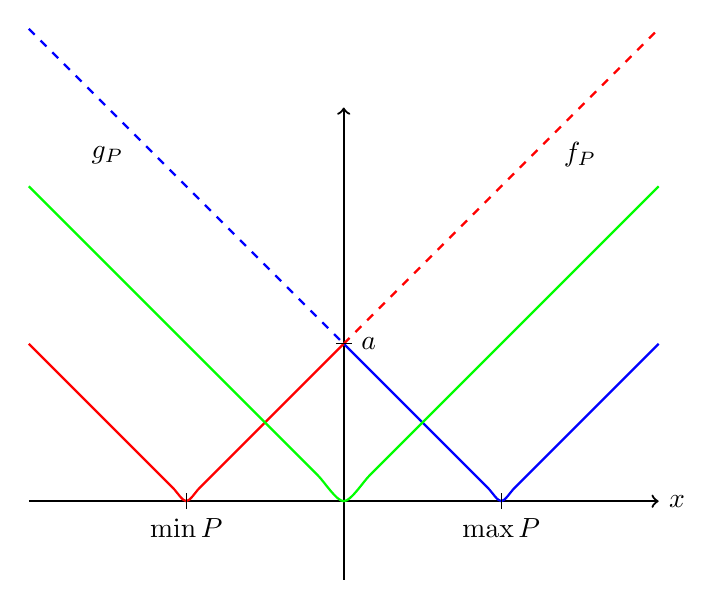
\begin{tikzpicture}[scale=2]
            % Axes
            \draw[thick, ->] (-2,0) -- (2,0) node[right] {$x$};
            \draw[thick, ->] (0,-0.5) -- (0,2.5);

            \draw[domain=-2:0, smooth, dashed, variable=\x, blue, thick] plot ({\x}, {abs(\x-1)});
            \draw[domain=0:2, smooth, dashed, variable=\x, red, thick] plot ({\x}, {abs(\x+1)});
            \draw[domain=0:2, smooth, variable=\x, blue, thick] plot ({\x}, {abs(\x-1)});
            \draw[domain=-2:0, smooth, variable=\x, red, thick] plot ({\x}, {abs(\x+1)});
            \draw[domain=-2:2, smooth, variable=\x, green, thick] plot ({\x}, {abs(\x)});

            % Indicate minima points
            \node[below] at (-1,-0.05) {$\min P$};
            \draw (-1, -0.05) -- (-1, 0.05);

            \node[below] at (1,-0.05) {$\max P$};
            \draw (1, -0.05) -- (1, 0.05);
            
            \draw (-0.05, 1) -- (0.05, 1);
            \node[right] at (0.05, 1) {$a$};
            \node at (-1.5, 2.2) {$g_P$};
            \node at (1.5, 2.2) {$f_P$};
        \end{tikzpicture}
        \caption{The GDFs $f_P$ (red), $g_P$ (blue) and $f_Q$ (green) for
            point clouds $P = \{-1, 1\}$ and $Q = \{0\}$.
            The minimum $h_P$ of the $f_P$ and $g_P$ is shown in solid lines.}
        \label{fig:min_max_stable_gdfs}
    \end{figure}

    Consider GDFs on $\R$ ($d = 1$).
    Fix a constant $a \in \R$ and let
    \begin{equation}
        f(P, x) = a \cdot |x - \min p| \quad \text{and} \quad g(P, x) = a \cdot |x - \max p|.
    \end{equation}
    The 0-dimensional persistence diagrams for these GDFs are
    $\dgm_0(f_P) = \{(0, \infty)\}$ and $\dgm_0(g_P) = \{(0, \infty)\}$ for any
    $P$, and thus are both $0$-stable.

    Consider $P = \{-1, 1\}$ and $Q = \{0\}$ with $d_H(P, Q) = 1$.
    As we can see in Figure~\ref{fig:min_max_stable_gdfs}, the 0-dimensional
    persistence diagrams of $h_P$ and $h_Q$ are
    \begin{align}
        \dgm_0(h_P) &= \{(0, a), (0, \infty)\}, \\
        \dgm_0(h_Q) &= \{(0, \infty)\}.
    \end{align}
    The cost of matching $(0, a)$ to $\Delta$ is $\frac{a}{2}$, so the
    bottleneck distance between the diagrams is $\frac{a}{2}$.
    Thus, for every $c \in [0, \infty)$ we can choose $a = 2c$ such that
    the stability constant of $h(P, x) = f(P, x) + g(P, x)$ is $c$.
    Thus, the minimum of two $0$-stable GDFs is not necessarily
    $c$-stable for any $c \in [0, \infty)$.
\end{example}

\todo{connect this theorem to the results above, something about how we can
trade the Lipschitz requirement for some other ones}

\begin{theorem}
    Let $f(P, x)$ and $g(P, x)$ be a $c_f$-stable GDF and a
    $c_g$-stable GDF with $q$-tame induced persistence modules $\mathbb{F}_P$ and
    $\mathbb{G}_P$ for all $P$. Let the sublevel sets of $f$ and $g$ be
    denoted as $f(P)_a = f^{-1}_P(-\infty, a]$ and
    $g(P)_a = g^{-1}_P(-\infty, a]$.
    % As $\mathbb{F}_P$ and $\mathbb{G}_P$ are $q$-tame, we have by
    % Theorem~\ref{thm:isometry} that
    % \begin{align}
    %     d_b(\dgm(f_P), \dgm(f_Q)) &= d_i(\mathbb{F}_P, \mathbb{F}_Q) \\
    %     d_b(\dgm(g_P), \dgm(g_Q)) &= d_i(\mathbb{G}_P, \mathbb{G}_Q).
    % \end{align}
    Let also
    \begin{align}
        d_i(\mathbb{F}_P, \mathbb{F}_Q) &= d_i(\{f(P)_a\}, \{f(Q)_a\}) \\
        d_i(\mathbb{G}_P, \mathbb{G}_Q) &= d_i(\{g(P)_a\}, \{g(Q)_a\}),
    \end{align}
    i.e. the interleaving maps for the persistence modules are induced by maps
    between filtrations of sublevel sets.
    Let those maps be denoted $\varphi^f_a : f(P)_a \to f(Q)_{a + c_f \cdot d_H(P, Q)}$,
    $\psi^f_a : f(Q)_a \to f(P)_{a + c_f \cdot d_H(P, Q)}$, and the same for $g$.
    Finally, we require three conditions:
    \begin{enumerate}
        \item $f(P, x) = g(P, x) \implies \varphi_a^f(x) = \varphi_a^g(x)$
        and $\psi_a^f(x) = \psi_a^g(x)$ for all $a \geq f(P, x)$.
        \item $f_P$ and $g_P$ are both continuous for all $P$.
        \item $f(P, x) \leq g(P, x) \implies f(Q, x) \leq g(Q, x)$
    \end{enumerate}
    Then the function $h(P, x) = \min\{f(P, x), g(P, x)\}$ is
    a $\max\{c_f, c_g\}$-stable GDF with $q$-tame induced persistence modules.
\end{theorem}
\begin{proof}
    \todo{}
\end{proof}

The results in this section concerning the pointwise minimum can be extended to
the pointwise maximum.
This is because $\max(A, B) = - \min( - A, - B)$, and negation preserves
stability by Lemma~\ref{lem:negation_stability}.
